\documentclass[12pt,a4paper]{report}
%\usepackage[utf8]{inputenc}
\usepackage{amsmath}


%\usepackage{amsfonts}
%\usepackage{amssymb}
\usepackage{xepersian}
\begin{document}
\section*{معادله لاپلاس دو بعدی با استفاده از روش گرادیان مزدوج }
معادله لاپلاس با استفاده از الگوریتم گرادیان مزدوج (\lr{CG}) حل شده و پتانسیل در نقاط درونی محاسبه شده است.
همچنین انرژی الکترواستاتیک محاسبه شده و با حل تحلیلی توسط متمتیکا مقایسه شده است.
با توجه به گام مکانی انتخاب شده که از مرتبه 
$O(10^{-2})$
است مقدار بدست آمده برای انرژی با استفاده از انتگرال گیری ذوزنقه ای تا رقم سوم اعشار با معنی است.

با افزایش تعداد نقاط گره در واقع تعداد نقاط مجهول در سیستم معادلات خطی افزایش می یابد و ماتریس بزرگتری باید محاسبه شود. از آنجا که نرخ همگرایی الگوریتم گرادیان مزدوج متناسب با جذر عدد حالت ماتریس حاصل است، با افزایش اندازه ماتریس عدد حالت بزرگتر شده و تعداد تکرارهای الگوریتم برای رسیدن به همگرایی افزایش می یابد.

 تعداد تکرارهای برنامه به ازای تعداد نقاط گره ای در راستای \lr{x} و \lr{y} در جدول زیر آورده شده است.

\begin{center}
\begin{tabular}{ |l|l|l|l|l| } 
 \hline
 \hline
 $n_x$ & $n_y$ & \ $dx,dy$ & \lr{iteration}\\ 
 \hline
 1000 & 10 & $0.1$ & 9 \\ 
 2000 & 20 & $5 \times 10^{-2} $ & 20 \\ 
 3000 & 30 & $3.3 \times 10^{-2}$ & 36 \\
 4000 & 40 & $2.5\times 10^{-2} $ & 52 \\
 \hline
 \hline
\end{tabular}
\end{center}

به نظر می رسد با ۲ برابر کردن تعداد نقاط گره در هر راستا تعداد تکرارها حدودا ۲ برابر می شود.
در هنگام محاسبات با افزایش تعداد گره ها معیار توقف هم به نسبت افزایش یافت.

در شکل های زیر نتایج حل عددی و حل تحلیلی به ترتیب مقایسه شده اند.

\centering
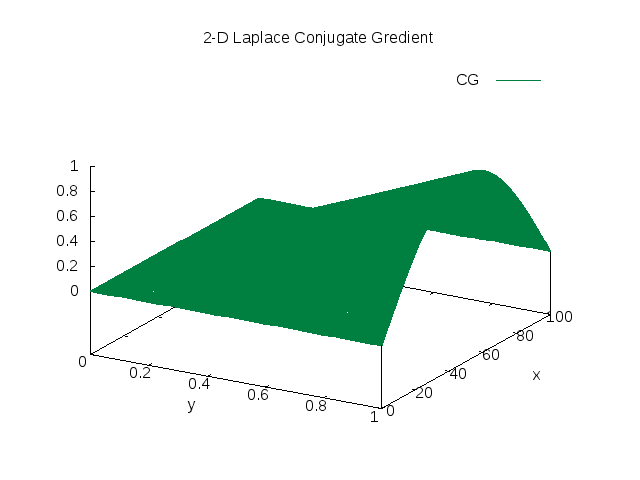
\includegraphics[scale=.8]{plot-1.png} 
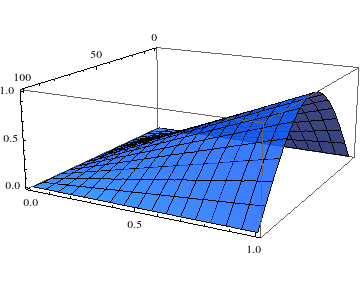
\includegraphics[scale=.8]{analytic.png} 







\end{document}